\documentclass{article}

\usepackage{amsmath, graphicx, makecell}
\graphicspath{ {./images/} }

\title{Ch. 22 CW \#2 Solutions}
\author{Principles of Microeconomics}
\date{\today}

\begin{document}

\maketitle

\begin{enumerate}

\item

	\begin{enumerate}
	
	\item Since cars and tires are perfect complements, Isabella's indifference curves create right angles.
	
		\begin{center}
		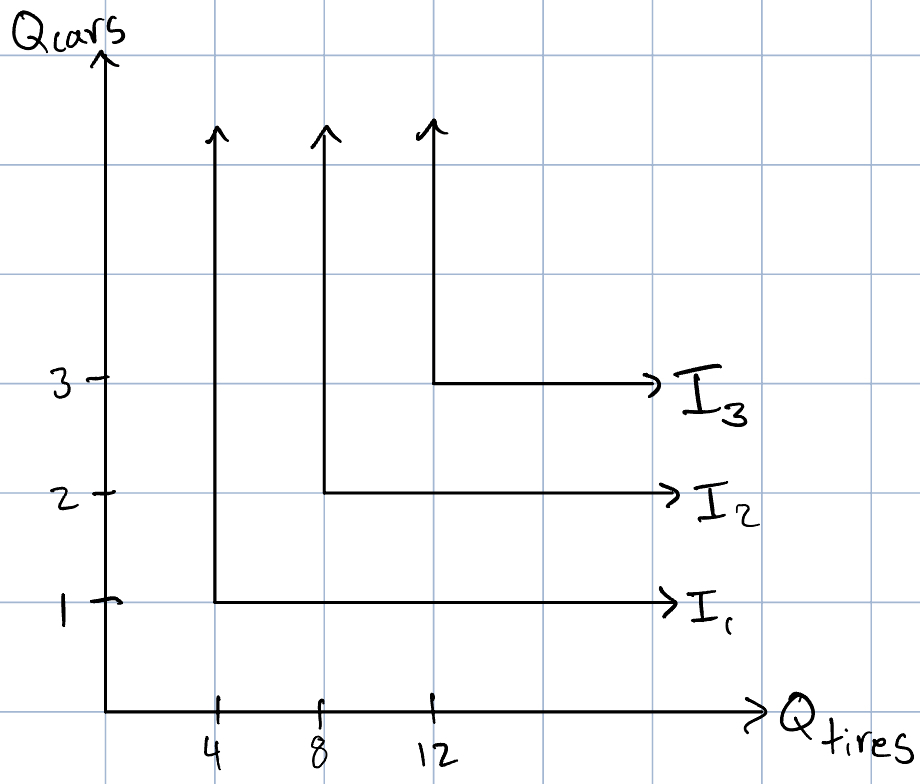
\includegraphics[width = 0.5\textwidth]{q1a}
		\end{center}
	
	\item Since Isabella gets utility only from her caffeine intake, she's always willing to trade off Valley Dew and cola at the same ratio, 1:2. That means they're perfect substitutes and her indifference curves are straight.
	
		\begin{center}
		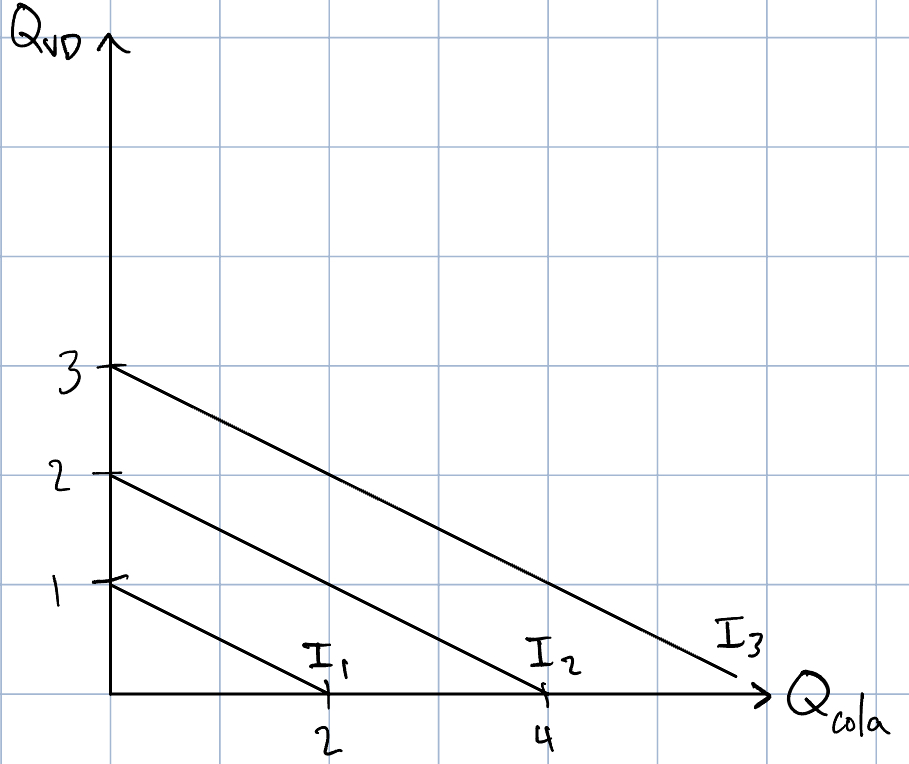
\includegraphics[width = 0.5\textwidth]{q1b}
		\end{center}
	
	\item Since both have diminishing marginal utility, her MRS will decrease as you move from left to right on her indifference curves. That means her indifference curves are curved.
	
		\begin{center}
		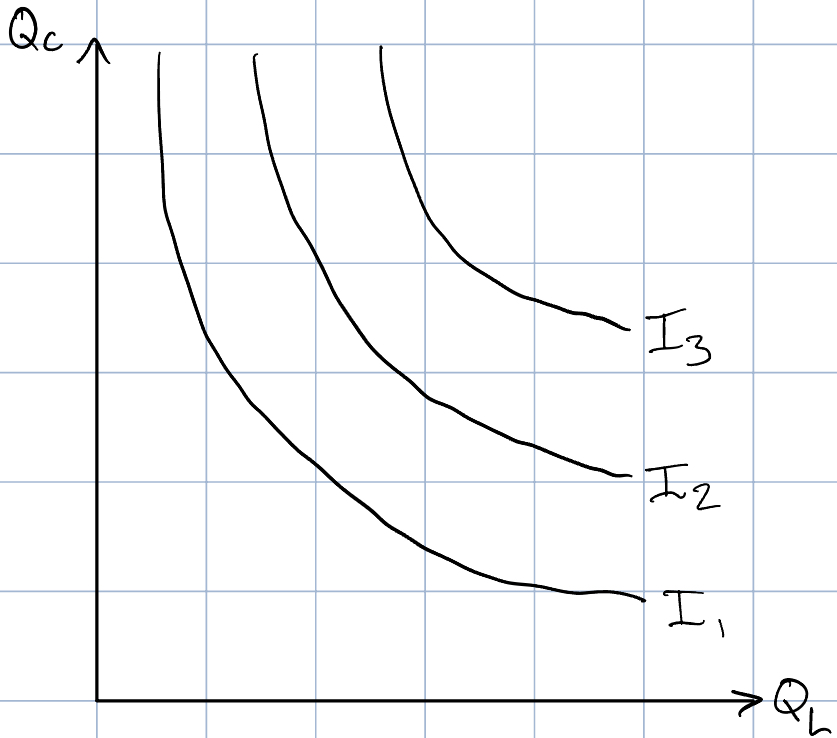
\includegraphics[width = 0.5\textwidth]{q1c}
		\end{center}
	
	\item Since she always wants to buy skis and bindings together, they are perfect complements, so her indifference curves create right angles.
	
		\begin{center}
		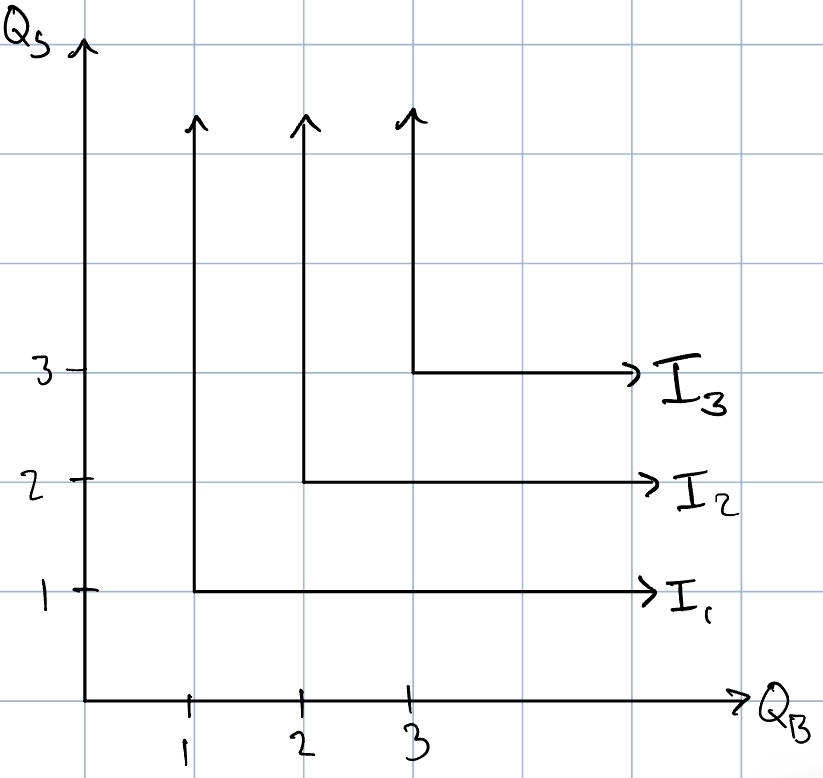
\includegraphics[width = 0.5\textwidth]{q1d}
		\end{center}
	
	\item Since water doesn't affect her utility, her indifference curves are horizontal lines.
	
		\begin{center}
		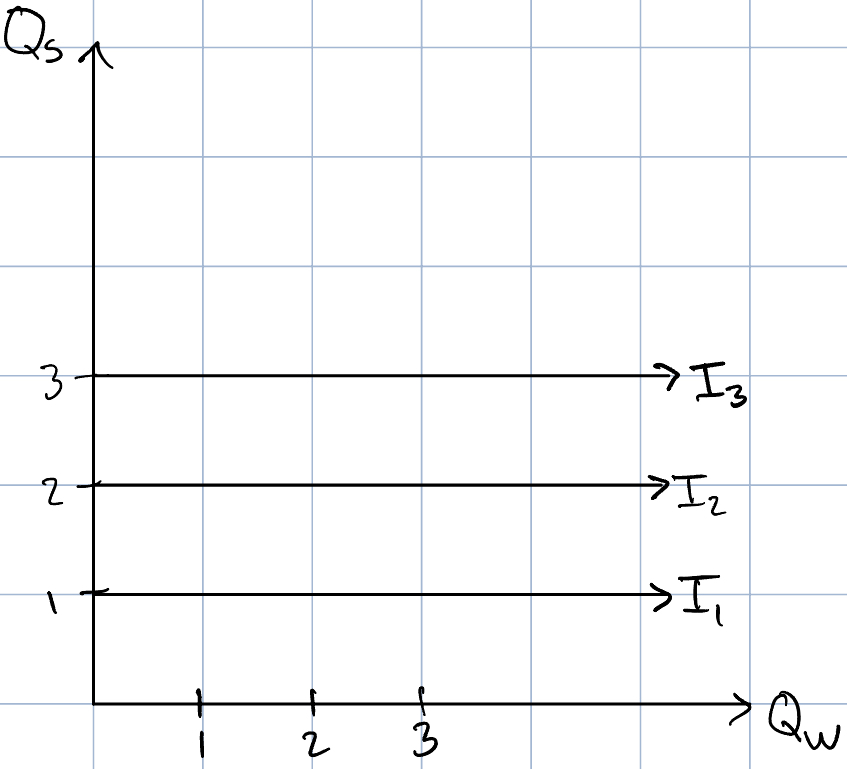
\includegraphics[width = 0.5\textwidth]{q1e}
		\end{center}
	
	\end{enumerate}
	
\item Diminishing marginal utility means that Marta gets less additional utility from each additional cup. That means her first cup gives her the most additional utility and her last cup gives her the least.

\item

	\begin{enumerate}
	
	\item The bundle gives Bridget and Erin utility levels of
	
		\begin{gather*}
		U_B(10, 5) = 10(10)(5) = 500 \\
		U_E(10,5) = 0.2(10^2)(5^2) = 500.
		\end{gather*}
		
		The bundles that give Bridget the same utility are defined by
		
		\begin{align*}
		500 &= 10FC \\
		50 &= FC \\
		C &= \frac{50}{F}.
		\end{align*}
		
		The bundles that give Erin the same utility are defined by
		
		\begin{align*}
		500 &= 0.2 F^2 C^2 \\
		2,500 &= F^2 C^2 \\
		50 &= F C \\
		C &= \frac{50}{F}
		\end{align*}
		
		Therefore, they have the same indifference curve through the point $(10,5)$. See (b) for the graphs.
	
	\item The bundle gives Bridget and Erin utility levels of
	
		\begin{gather*}
		U_B(15,8) = 10(15)(8) = 1,200 \\
		U_E(15, 8) = 0.2(15^2)(8)^2 = 2,880
		\end{gather*}
		
		The bundles that give Bridget the same utility are defined by
		
		\begin{align*}
		1,200 &= 10FC \\
		120 &= FC \\
		C &= \frac{120}{F}
		\end{align*}
		
		The bundles that give Erin the same utility are defined by 
		
		\begin{align*}
		2,880 &= 0.2F^2C^2 \\
		14,400 &= F^2 C^2 \\
		120 &= F C \\
		C &= \frac{120}{F}
		\end{align*}
		
		Once again, Bridget and Erin have the same indifference curve.
		
		\begin{center}
		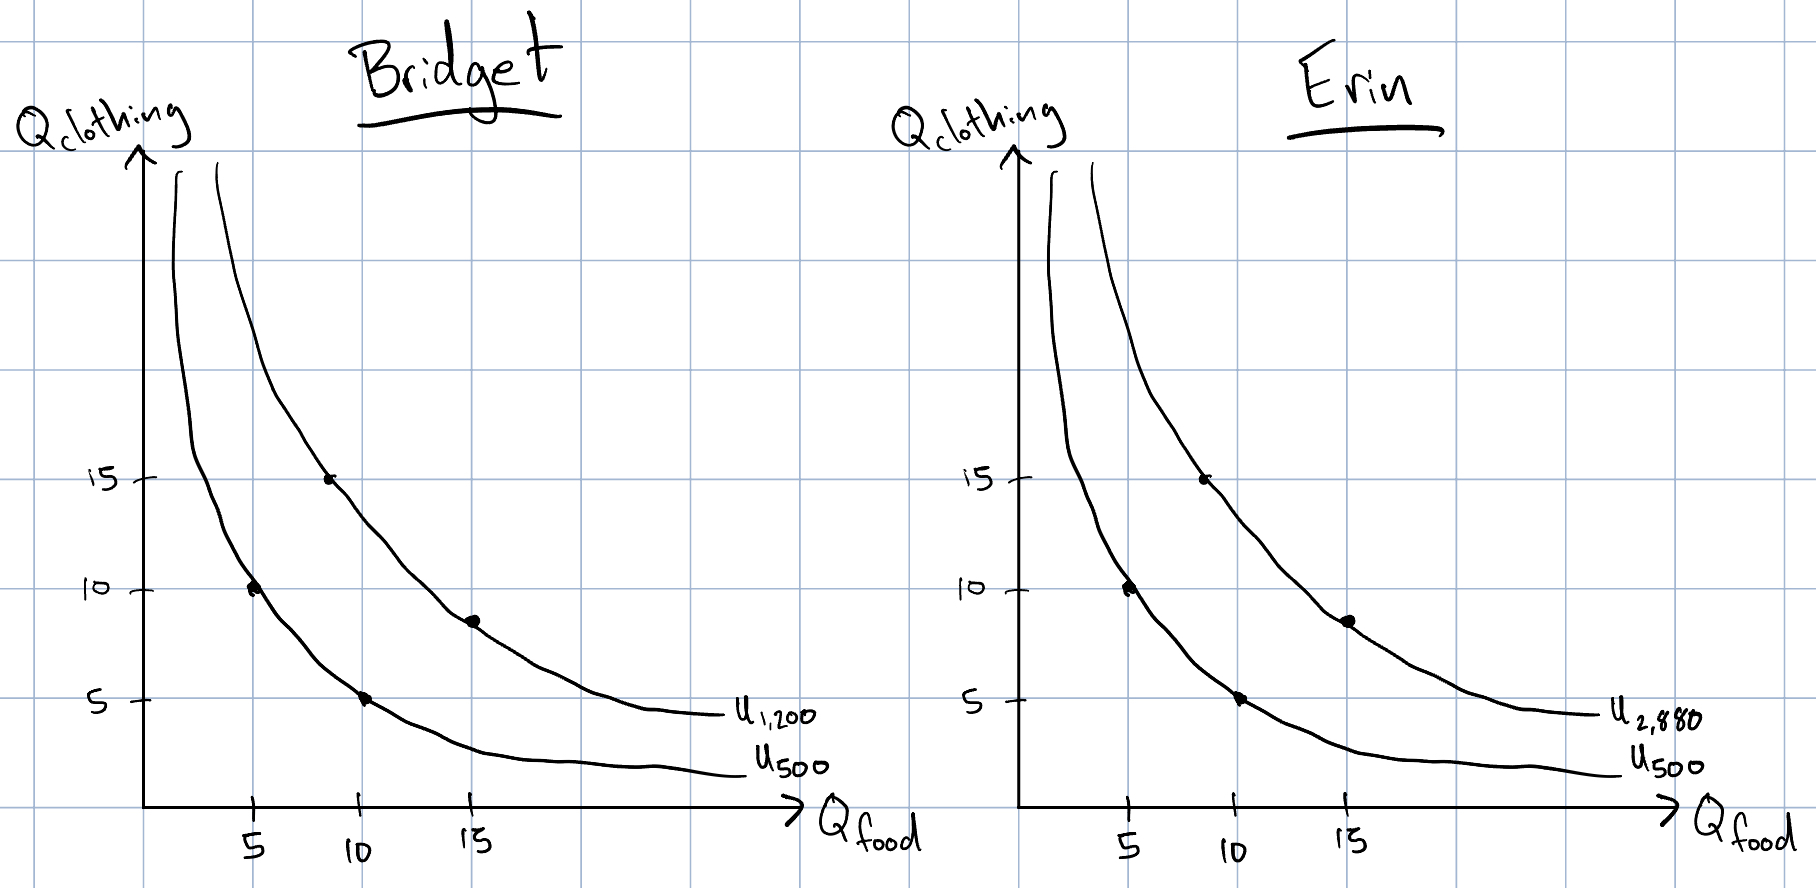
\includegraphics[width = \textwidth]{q3}
		\end{center}
	
	\item I think they have the same preferences because they appear to have the same indifference curves. If you're looking for a challenge, it's possible to prove they have the same indifference curve running through an arbitrary bundle $(F_1, C_1)$.
	
	\end{enumerate}
	
\item
	
	\begin{enumerate}
	
	\item Julius's budget constraint is $200 = 20 Q_M + 4 Q_T$. At his optimal bundle, his MRS equals the (negative) slope of his budget constraint. Therefore, $MRS = 5$.
	
		\begin{center}
		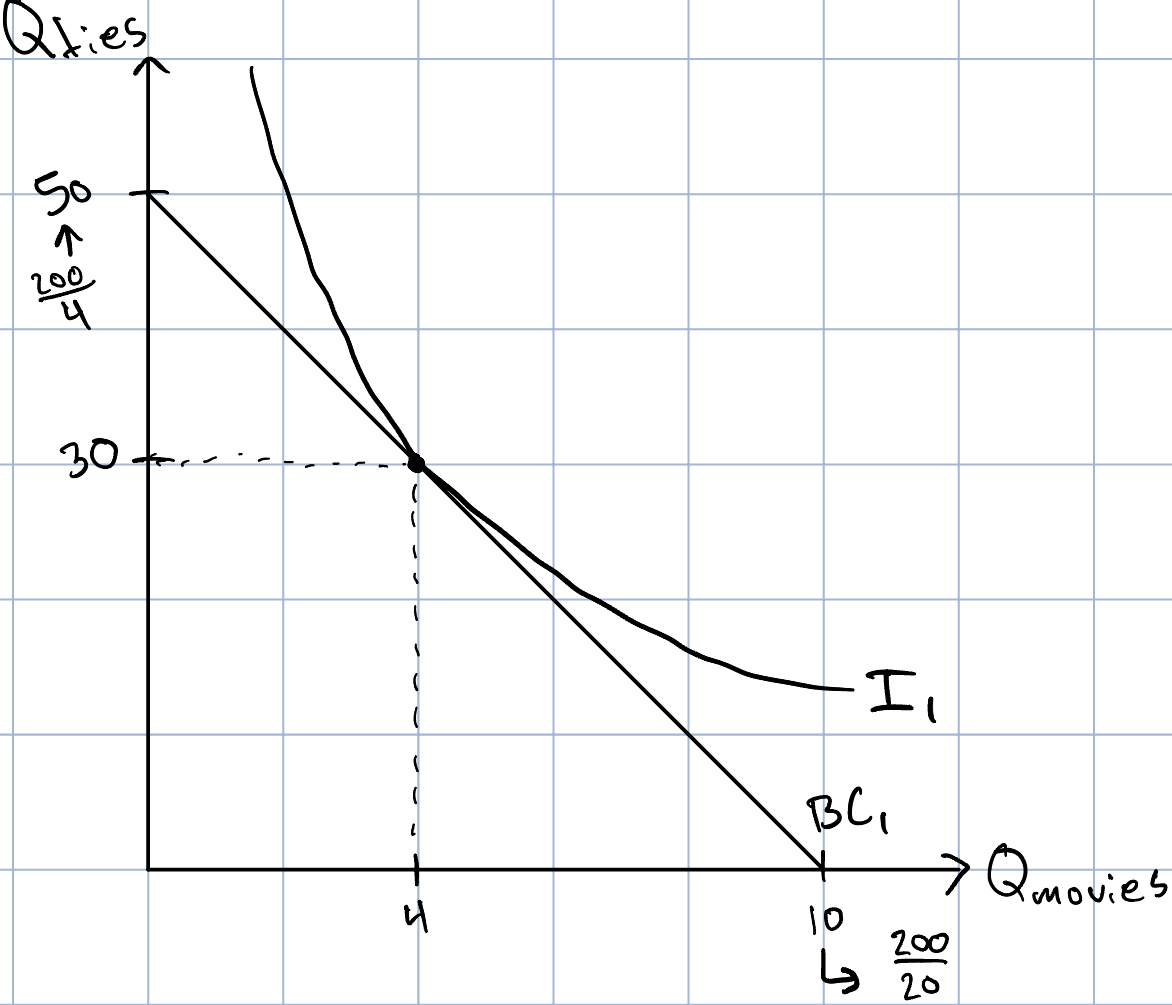
\includegraphics[width = 0.5\textwidth]{q4a}
		\end{center}
	
	\item I assume that movies and ties are normal goods, so when Julius's budget doubles, he's going to consume more of both.
	
		\begin{center}
		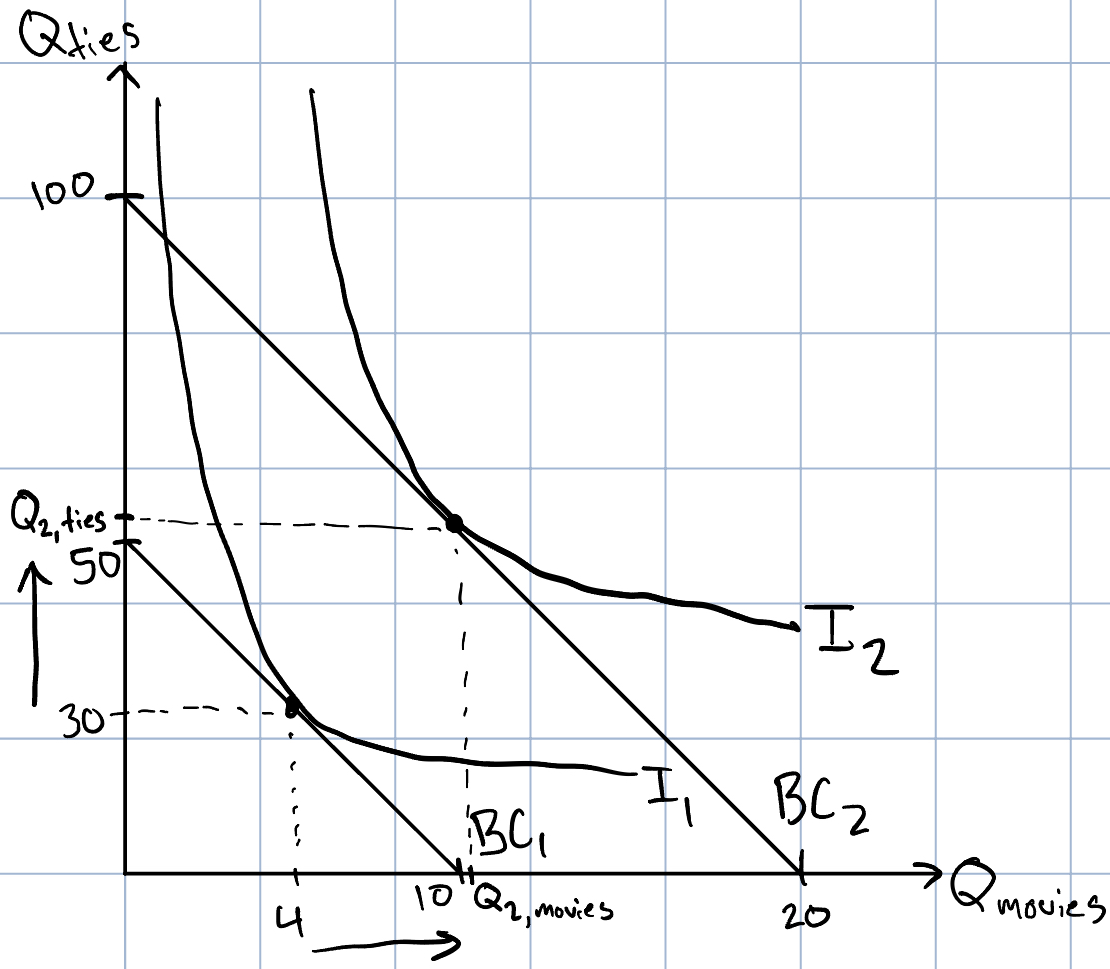
\includegraphics[width = 0.5\textwidth]{q4b}
		\end{center}
		
	\item The quantity of ties he consumes will unambiguously decrease. Since the relative price of ties increases, he will substitute away from ties and towards movies. Since his purchasing power decreases and ties are a normal good, he will consume fewer ties. The income and substitution effects are both negative.
	
	As I've drawn it, the quantity of movies he consumes will decrease, but it's ambiguous. The income effect is negative because movies are a normal good, but the substitution effect is positive because movies become cheaper relative to ties. The overall effect of the price increase will depend on whether the income effect or the substitution effect is bigger. In my drawing, the income effect is bigger.
	
	\begin{center}
	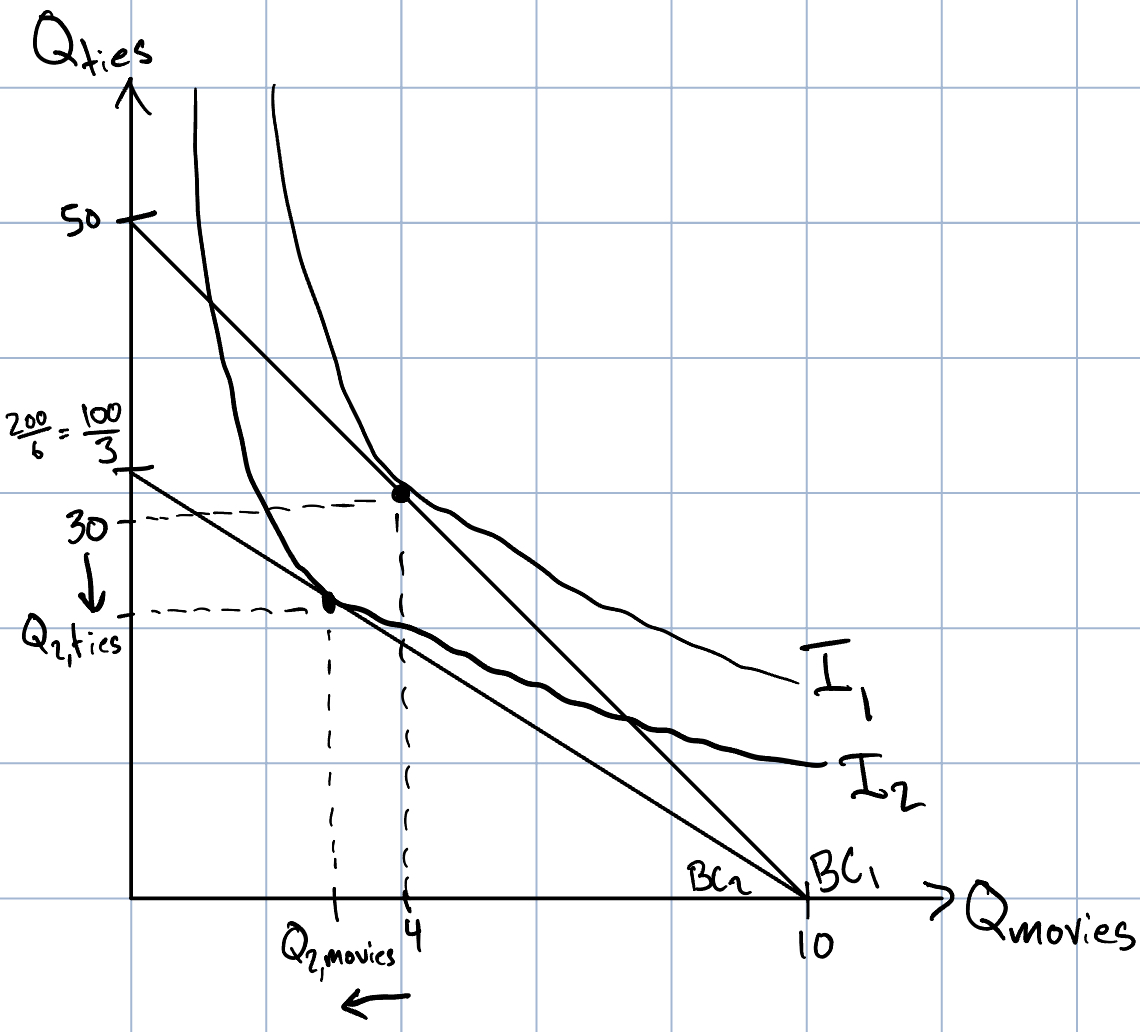
\includegraphics[width = 0.5\textwidth]{q4c}
	\end{center} 
	
	\end{enumerate}
	
\item

	\begin{enumerate}
	
	\item Bernie can consume the bundles defined by $20 = 4Q_N + 2Q_P$.
	
		\begin{center}
		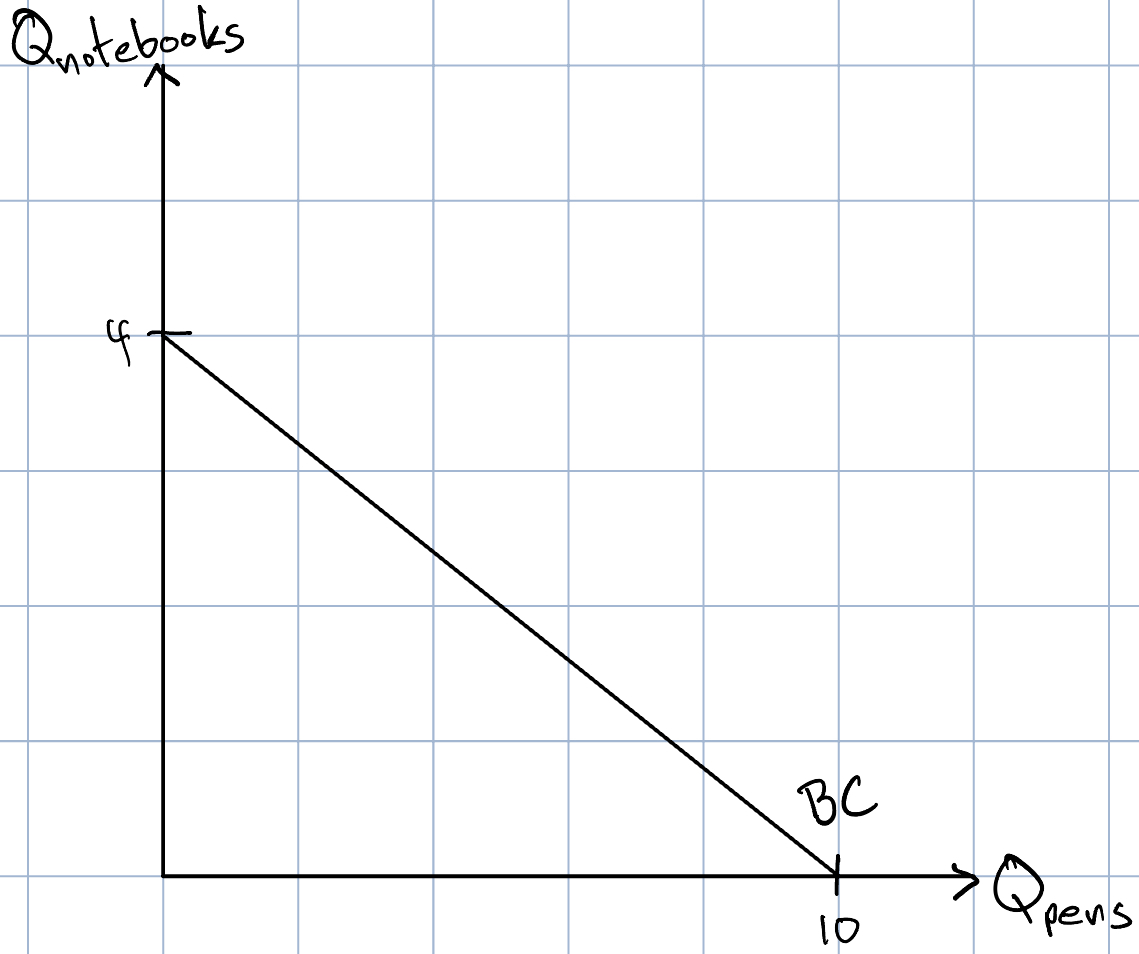
\includegraphics[width = 0.5\textwidth]{q5a}
		\end{center}
	
	\item 
	
		\begin{center}
		\begin{tabular}{c c | c c}
		\makecell{Quantity of\\Notebooks} & \makecell{Utility from\\Notebooks} & \makecell{Marginal\\Utility} & \makecell{Marginal Utility\\per Dollar} \\
		\hline
		0 & 0 &-- & -- \\
		1 & 32 & 32 & 8 \\
		2 & 60 & 28 & 7 \\
		3 & 84 & 24 & 6 \\
		4 & 104 & 20 & 5 \\
		5 & 120 & 26 & 4
		\end{tabular}

		\begin{tabular}{c c | c c}
		\makecell{Quantity of\\Pens} & \makecell{Utility from\\Pens} & \makecell{Marginal\\Utility} & \makecell{Marginal Utility\\per Dollar} \\
		\hline
		0 & 0 &-- & -- \\
		2 & 28 & 14 &  7\\
		4 & 52 & 12 & 6 \\
		6 & 72 & 10 & 5 \\
		8 & 88 & 8 & 4 \\
		10 & 100 & 6 & 3 \\
		\end{tabular}
		\end{center}
	
	\item Bernie will buy 3 notebooks and 4 pens because that's the bundle that equalizes marginal utility per dollar across the two goods and that lies on his budget constraint.
	
	\end{enumerate}

\end{enumerate}

\end{document}